\documentclass[TFG.tex]{subfiles}

\begin{document}

%\hyphenation{equi-va-len-cia}\hyphenation{pro-pie-dad}\hyphenation{res-pec-ti-va-men-te}\hyphenation{sub-es-pa-cio}
\chapter{Preliminares}

%ME QUIERO ASEGURAR MEJOR DE LO DE QUE SE PUEDEN CONSIDERAR SIEMPRE NÚMERO FINITO DE CRUCES Y TAL
Aunque el término \emph{grupo de trenzas} fue acuñado por Artin en 1925 \cite{ArtinA}, estos grupos ya fueron considerados por Hurwitz en 1891 \cite{Hur} como lo que en terminología moderna se llamaría ``grupo fundamental de espacios de configuración de $n$ puntos en el plano complejo''. Magnus en 1935 \cite{Magnus} consideró el mismo grupo desde el punto de vista de los \emph{mapping classes}. Markov \cite{Markoff} dio una aproximación totalmente algebraica. 

En este capítulo veremos varias de estas definiciones, que son todas equivalentes \cite{Zariski}, ya que una sola definición no es suficiente para enunciar y demostrar los resultados que se presentan en el resto del trabajo. Esta variedad de definiciones permite estudiar los grupos de trenzas desde perspectivas muy distintas, lo cual aporta una gran riqueza a la teoría.


\section{Trenzas como colección de cuerdas}
Empezamos dando la definición más gráfica e intuitiva, consistente en visualizar las trenzas como cuerdas que se entrelazan. 

\begin{defi}\label{geo}
Sea $n\geq 1$ un entero. Denotemos $\Sigma_n$ al grupo simétrico sobre $n$ elementos. Sean $n$ puntos $P_1,\dots, P_n$ en $\C$ (se puede suponer que $P_k=k$ para todo $1\leq k\leq n$). Se define la \emph{trenza geométrica de $n$ cuerdas} como la $n$-upla $\beta=(\beta_1,\dots,\beta_n)$ de caminos $\beta_k:[0,1]\to\C\times[0,1]$ tal que:
\begin{itemize}
\item $\beta_k(t)=(\alpha_k(t),t)$, donde $\alpha_k(0)=P_k$ para todo $1\leq k\leq n$, 
\item existe una permutación $\tau=\tau(\beta)\in\Sigma_n$ tal que $\alpha_k(1)=P_{\tau(k)}$ para todo $1\leq k\leq n$, llamada \emph{permutación inducida por $\beta$},
\item $\alpha_k(t)\neq \alpha_l(t)$ para todo $k\neq l$ y para todo $t\in[0,1]$.
\end{itemize}
Si la permutación inducida por $\beta$ es el elemento neutro de $\Sigma_n$, es decir, si $\beta_k(1)=(P_k,1)$ para todo $1\leq k\leq n$, entonces decimos que la trenza geométrica es \emph{pura}.

Dos trenzas geométricas $\alpha$ y $\beta$ se dicen \emph{homotópicas} si existe una familia continua de trenzas $\{\gamma_s\}_{s\in[0,1]}$ de modo que $\gamma_0=\alpha$ y $\gamma_1=\beta$. Es decir, dos trenzas geométricas son homotópicas si son homotópicas como colección de caminos relativamente a los puntos extremos. Consideraremos que dos trenzas geométricas son la misma si son homotópicas, y a la clase de homotopía de una trenza geométrica de $n$ cuerdas la llamaremos \emph{trenza de $n$ cuerdas}. Nótese que si $\alpha$ y $\beta$ son homotópicas entonces $\tau(\alpha)=\tau(\beta)$, así que diremos que una trenza es \emph{pura} si los elementos de su clase de homotopía son trenzas geométricas puras.
\end{defi}

El dibujo tridimensional de una trenza geométrica tiene la siguiente forma:
\begin{figure}[h!]
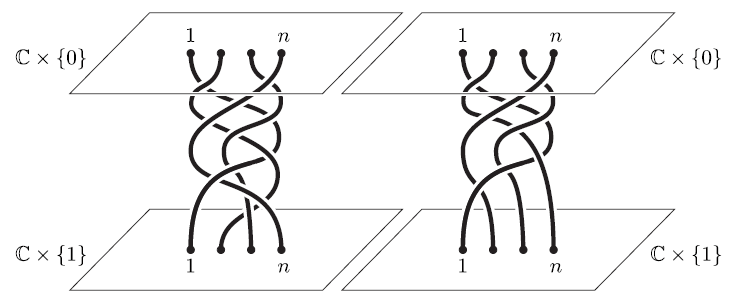
\includegraphics[scale=0.7]{Imagenes/hilos}
\caption{Una trenza geométrica pura y una trenza geométrica no pura.}\label{hilos}
\end{figure}
%para conseguir cambiar la permutación habría que cortar un hilo porque los puntos finales no se pueden mover. 

%La manera más usual de representar las trenzas puras es representar el movimiento de $n$ puntos en un dibujo tridimensional. Para cada $t\in[0,1]$ se representa la $n$-upla $\beta(t)=(\beta_1(t),\dots,\beta_n(t))$ simplemente dibujando en $\C\times[0,1]$ los $n$ puntos $(\beta_1(t),t),\dots,(\beta_n(t),t)$, con la condición de que dos de estos puntos nunca son iguales y de que $\beta_i(0)=\beta_i(1)$ para todo $i=1,\dots, n$.
\begin{observacion}
Para cada $t\in[0,1]$, el plano $\C\times\{t\}$ es atravesado una sola vez por cada cuerda de la trenza. 
\end{observacion}

Normalmente, se representan las trenzas como su proyección en $\R\times[0,1]$ (posiblemente seguida de una rotación de 90º). Los puntos en los que la proyección de dos cuerdas coincida los representaremos como en la Figura \ref{cruce} para conservar la información de cuál cruzaba originalmente por encima. Salvo homotopía, podemos suponer que la proyección tiene un número finito de puntos de cruce, en los cuales solo intervienen dos cuerdas. Además podemos suponer también que los cruces ocurren a distintas alturas, es decir, para distintos valores de $t\in[0,1]$. En la Figura \ref{plana} se ilustra la proyección de la trenza no pura de la Figura \ref{hilos}. 
\begin{figure}[h!]
\centering
\begin{tikzpicture}
\braid[ number of strands=3, %lower bound
 border height=2pt,style strands={1}{line width=2pt},style strands={2}{line width=2pt},style strands={3}{draw=none}] (braid) at (1,0)%optional, it's a name
          a_1^{-1};
\end{tikzpicture}
\begin{tikzpicture}
\braid[ number of strands=3, %lower bound
 border height=2pt,style strands={3}{line width=2pt},style strands={2}{line width=2pt}, style strands={1}{draw=none}] (braid) at (1,0)%optional, it's a name
          a_2;
\end{tikzpicture}

\caption{Cruce positivo y cruce negativo, respectivamente.}\label{cruce}
\end{figure}

\begin{defi}\label{estandar}
Se definen los \emph{generadores estándar} o \emph{generadores de Artin} como las trenzas $\sigma_i$ con $1\leq i\leq n-1$ indicadas en la Figura \ref{artingen}.
\begin{figure}[h!]
\begin{tikzpicture}
\fill[black] ( 6.7 , -0.5 ) circle ( 1 pt ) ;
\fill[black] ( 7 , -0.5 ) circle ( 1 pt ) ;
\fill[black] ( 7.3 , -0.5 ) circle ( 1 pt ) ;

\fill[black] ( 1.7 , -0.5 ) circle ( 1 pt ) ;
\fill[black] ( 2 , -0.5 ) circle ( 1 pt ) ;
\fill[black] ( 2.3 , -0.5 ) circle ( 1 pt ) ;
\braid[ number of strands=8, %lower bound
 border height=2pt,style strands={8}{line width=2pt}, style strands={7}{draw=none},style strands={6}{line width=2pt},style strands={5}{line width=2pt},style strands={4}{line width=2pt},style strands={3}{line width=2pt}, style strands={2}{draw=none},style strands={1}{line width=2pt}] (braid) at (1,0)%optional, it's a name
          a_4^{-1};
          \node[ at=(braid-4-s),  label=north :  $i$ ] {} ;
\node[ at=(braid-5-s),  label=north : $i+1$ ] {} ;
\draw (4.5,-2) node[anchor=south] {$\sigma_i$};
\end{tikzpicture}

\begin{tikzpicture}
\fill[black] ( 6.7 , -0.5 ) circle ( 1 pt ) ;
\fill[black] ( 7 , -0.5 ) circle ( 1 pt ) ;
\fill[black] ( 7.3 , -0.5 ) circle ( 1 pt ) ;

\fill[black] ( 1.7 , -0.5 ) circle ( 1 pt ) ;
\fill[black] ( 2 , -0.5 ) circle ( 1 pt ) ;
\fill[black] ( 2.3 , -0.5 ) circle ( 1 pt ) ;
\braid[ number of strands=8, %lower bound
 border height=2pt,style strands={8}{line width=2pt}, style strands={7}{draw=none},style strands={6}{line width=2pt},style strands={5}{line width=2pt},style strands={4}{line width=2pt},style strands={3}{line width=2pt}, style strands={2}{draw=none},style strands={1}{line width=2pt}] (braid) at (1,0)%optional, it's a name
          a_4;
          \node[ at=(braid-4-s),  label=north :  $i$ ] {} ;
\node[ at=(braid-5-s),  label=north : $i+1$ ] {} ;
\draw (4.5,-2) node[anchor=south] {$\sigma_i^{-1}$};
\end{tikzpicture}
\caption{Generador de Artin y su inverso.}\label{artingen}
\end{figure}
\end{defi}\

A partir de las observaciones anteriores, es claro que cualquier trenza se puede construir como concatenación de los generadores de Artin.

\begin{figure}[h!]
\centering
\begin{tikzpicture}
\draw [line width=1.5pt, dash pattern=on 4pt off 4pt] (0,0.9)-- (0,4.2);
\draw (-0.7,0.7) node[anchor=north west] {$\mathbb{R}\times\{0\}$};
\draw [line width=1.5pt, dash pattern=on 4pt off 4pt] (9.1,0.9)-- (9.1,4.2);
\draw (8.4,0.7) node[anchor=north west] {$\mathbb{R}\times\{1\}$};
\braid[rotate=90, number of strands=4, %lower bound
 border height=2pt,style strands={1}{line width=2pt},style strands={2}{line width=2pt},style strands={3}{line width=2pt},style strands={4}{line width=2pt}, style floors={1}{dashed}] (braid) at (1,0)%optional, it's a name
          a_1^{-1}a_3^{-1}a_2^{-1}a_1^{-1}a_3^{-1}a_2^{-1}a_3a_2^{-1}a_1^{-1};
\node[ at=(braid-1-s),  label=west : 1 ] {} ;
\node[ at=(braid-4-s),  label=west : $n$ ] {} ;
\node[ at=(braid-1-e),  label=east : 1 ] {} ;
\node[ at=(braid-2-e),  label=east : $n$ ] {} ;
\end{tikzpicture}
\caption{Ejemplo de representación plana.}\label{plana}
\end{figure}




\subsection{Estructura de grupo}
Una de las características más importantes del conjunto de clases de homotopía de trenzas es que puede dotarse de estructura de grupo para cada $n$. Para ello, definiremos el producto de trenzas. 

\begin{defi}
El producto de dos trenzas $\alpha=(\alpha_1,\dots, \alpha_n)$ y $\beta=(\beta_1,\dots,\beta_n)$ se define como la trenza
$$\alpha\cdot\beta = (\alpha_1\beta_{\tau(1)},\dots, \alpha_n\beta_{\tau(n)}),$$
donde $\tau=\tau(\alpha)$. Es decir, el producto de dos trenzas en el mismo número de cuerdas es su concatenación, en la cual se recorre en primer lugar $\alpha$ y después $\beta$. En la Figura \ref{producto} se ilustra un ejemplo. En ocasiones omitiremos el punto y escribiremos simplemente $\alpha\beta$. Asimismo, denotaremos $\alpha^n=\underbrace{\alpha\cdots\alpha}_{n\text{ veces}}$.
\end{defi}

\begin{figure}[h!]
\centering
%\begin{center}
\resizebox{7cm}{2.cm}{%
\begin{tikzpicture}
\braid[ rotate=90, number of strands=3, %lower bound
 border height=2pt,style strands={1}{line width=1.5pt},style strands={2}{line width=1.5pt},style strands={3}{line width=1.5pt}] (braid) at (1,1.5)%optional, it's a name
          a_2^{-1}a_1a_2^{-1};
         \fill[ black ] ( 2 , 2 ) circle (2 pt ) ;
\end{tikzpicture}
\begin{tikzpicture}
\braid[ rotate=90, number of strands=3, %lower bound
 border height=2pt,style strands={1}{line width=1.5pt},style strands={2}{line width=1.5pt},style strands={3}{line width=1.5pt}] (braid) at (1,0)%optional, it's a name
          a_2a_2a_1^{-1};
          \draw (3.5,2.2) node[anchor=north west] {\Large=};
\end{tikzpicture}
}
%\end{center}
\end{figure}
\begin{figure}[h!]
\resizebox{10cm}{2.3cm}{%
\begin{tikzpicture}
\braid[ rotate = 90, number of strands=3, %lower bound
 border height=2pt,style strands={1}{line width=1.5pt},style strands={2}{line width=1.5pt},style strands={3}{line width=1.5pt}] (braid) at (1,2)%optional, it's a name
          a_2^{-1}a_1a_2^{-1}a_2a_2a_1^{-1};
           \draw (4.3,2.2) node[anchor=north west] {\Large=};
            \fill[ black ] ( 1.1 , 3 ) circle (2.3 pt ) ;
            \fill[ black ] ( 1.1 , 2 ) circle (2.3 pt ) ;
            \fill[ black ] ( 1.1 , 1 ) circle (2.3 pt ) ;
            \draw [rotate around={90.:(1.1,2.5)},line width=1.5pt,dotted] (1.1,2.5) ellipse (0.7843018170151402cm and 0.6442593318876021cm);
\end{tikzpicture}\begin{tikzpicture}
%\clip (0,-2) rectangle (4, -8);
\braid[ rotate=90, number of strands=3, %lower bound
 border height=2pt,style strands={1}{line width=1.5pt},style strands={2}{line width=1.5pt},style strands={3}{line width=1.5pt}] (braid) at (1,3)%optional, it's a name
          a_2^{-1}a_1a_2a_1^{-1};
\end{tikzpicture}
}
\caption{Producto de dos trenzas.}\label{producto}
\end{figure}


Denotemos $B_n$ al conjunto de clases de homotopía de trenzas de $n$ cuerdas y $PB_n$ al conjunto de clases de homotopía de trenzas puras de $n$ cuerdas. Es evidente que la multiplicación anterior induce una operación en $B_n$ (y por tanto en $PB_n)$; es más, se tiene el siguiente resultado.

\begin{prop}
El conjunto $B_n$ dotado de esta operación tiene estructura de grupo, y se le llama \emph{grupo de trenzas de $n$ cuerdas}. El resultado también es cierto para $PB_n$, cuyo nombre es \emph{grupo de trenzas puras de $n$ cuerdas}. 
\end{prop}

\begin{dem}
Sean $\alpha$ y $\beta$ dos trenzas con representantes $a=(a_1,\dots, a_n)$ y $b=(b_1,\dots, b_n)$ respectivamente. En primer lugar, veamos que la operación está bien definida, es decir, que $a\cdot b$ es una trenza, y por tanto podemos definir $\alpha\beta=[a\cdot b]$. Sea $\tau=\tau(a)$ la permutación inducida por $a$. Como $a_kb_{\tau(k)}(0)=a_k(0)=(P_k,0)$ para todo $1\leq k\leq n$, se cumple la primera propiedad de la Definición \ref{geo}. Para la segunda, basta observar que la nueva permutación es $\tau(a\cdot b)=\tau(b)\circ \tau(a)$. En particular, si $a$ y $b$ son puras, entonces la permutación inducida por el producto también es la identidad, por lo que el producto es una trenza pura. Por último, si $t\in[0,1/2]$, entonces $a_k\beta_{\tau(k)}=a_k(2t)$ y si $t\in [1/2,1]$, $\alpha_k\beta_{\tau(k)}=\beta_{\tau(k)}(2t-1)$ para todo $1\leq k\leq n$, por lo que se tiene claramente la tercera propiedad. 

Por otra parte, si $a'$ y $b'$ son otros representantes de $\alpha$ y $\beta$ respectivamente, se tiene que $[a'\cdot b']=[a\cdot b]$ por las propiedades de la homotopía de caminos con respecto a la concatenación.

Veamos ahora la estructura de grupo. Tenemos que probar que la operación es asociativa, pero esto se deduce de que la concatenación de caminos es asociativa salvo homotopía.
Tenemos claramente que la identidad es la trenza constante representada por $Id=(Id_1,\dots, Id_n)$, donde $Id_k$ denota el camino $(P_k, t)$ para $t\in[0,1]$ y para $1\leq k\leq n$.
Finalmente, dada $\alpha=[(a_1,\dots, a_n)]$ con permutación inducida $\tau$, se tiene que $\alpha^{-1}=[(\overline{a}_{\tau^{-1}(1)},\dots, \overline{a}_{\tau^{-1}(n)})]$, donde $\overline{a}_k$ denota el camino que es opuesto a $a_k$ en la primera coordenada y que es idéntico a $a_k$ en la segunda coordenada. 

En efecto, usando las propiedades de la homotopía de caminos con respecto al camino opuesto:
\[
\alpha\alpha^{-1}=[(a_1,\dots, a_n)\cdot (\overline{a}_{\tau^{-1}(1)},\dots, \overline{a}_{\tau^{-1}(n)})]=[(a_1\overline{a}_{\tau(\tau^{-1}(1))},\dots, a_n\overline{a}_{\tau(\tau^{-1}(n))})]=[Id]
\]

Análogamente se prueba $\alpha^{-1}\alpha=[Id]$. 
$\QED$
\end{dem}


\begin{figure}[h!]
\begin{tikzpicture}
\clip (0,-1) rectangle (5.5, 2.1);
\braid[ rotate=90, number of strands=3, %lower bound
 border height=2pt,style strands={1}{line width=1.5pt},style strands={2}{line width=1.5pt},style strands={3}{line width=1.5}, style all floors={}] (braid) at (0,-1)%optional, it's a name
          a_2^{-1}a_2^{-1}a_1a_2^{-1} ;
\draw (3,-1) node[anchor=south] {$\beta$};
\end{tikzpicture}
\begin{tikzpicture}
\clip (0.5,-1) rectangle (6, 2.1);
\braid[ rotate=90, number of strands=3, %lower bound
 border height=2pt,style strands={3}{line width=1.5pt},style strands={2}{line width=1.5pt}, style strands={1}{line width=1.5pt}] (braid) at (0,-1)%optional, it's a name
          a_2a_1^{-1}a_2a_2;
\draw (3.2,-1) node[anchor=south] {$\beta^{-1}$};
\end{tikzpicture}
\caption{Inversa de una trenza.}\label{especular}
\end{figure}


\section{Espacios de configuración}
Vamos a empezar dando la noción general de espacio de configuración, introducida por Fadell en 1962 \cite{Fadell}.
\begin{defi}
Dado un espacio topológico $X$, el $n$-ésimo \emph{espacio de configuración} de $X$ o \emph{espacio de configuración de $n$ puntos} de $X$ se define como el conjunto
$$M_n(X)=\{(x_1,\dots,x_n)\in X^n\mid x_i\neq x_j\ \forall i\neq j\},$$
dotado de la topología de subsespacio de $X^n$. Cuando el espacio topológico $X$ se sobreentienda por el contexto, el espacio de configuración se denotará simplemente $M_n$. 
\end{defi}

Hay una acción natural del grupo simétrico $\Sigma_n$ en los puntos de $M_n(X)$ dada por 
\begin{gather*}
\Sigma_n\times M_n(X)\to M_n(x)\\
\ (\sigma,x)\mapsto \sigma(x).
\end{gather*}
Esto da lugar al espacio definido a continuación:
\begin{defi}
Se define el $n$-ésimo \emph{espacio de configuración no ordenado} de $X$ o \emph{espacio de configuración de $n$ puntos no ordenados} de $X$ como 
$$N_n(X)=M_n(X)/\Sigma_n,$$
es decir, el espacio de órbitas de la acción. De igual manera que con el anterior espacio de configuración, cuando se sobreentienda $X$, lo denotaremos por $N_n$. 
\end{defi}

\begin{observacion}
Para cualquier espacio topológico $X$, $M_1(X)=N_1(X)=X$.
\end{observacion}

\begin{ej}
Veamos un ejemplo no trivial de espacio de configuración. Consideremos $M_2(\R^3)=\{(x_1,x_2)\in\R^3\times\R^3\mid x_1\neq x_2\}$. Podemos definir la aplicación $M_2(\R^3)\to \R^3\times(\R^3\setminus\{0\})$ como
\[
(x_1,x_2)\mapsto (x_1+x_2,x_1-x_2).
\]
Es fácil ver que esta aplicación es un homeomorfismo, por lo que $M_2(\R^3)\cong \R^3\times(\R^3\setminus\{0\})$. Además, la aplicación es compatible con la acción de $\Sigma_2$, es decir, la aplicación sigue siendo un homeomorfismo sobre $\R^3\times(\R^3\setminus\{0\})$ al permutar las componentes. Sin embargo, punto a punto, lo que se observa es que la primera coordenada se conserva y la segunda cambia de signo tras la permutación. Por lo tanto, en $N_2(\R^3)=M_2(\R^3)/\Sigma_2$, $(x,y)\sim (x,-y)$ y no hay más puntos distintos relacionados entre sí. Por tanto, $N_2(\R^3)=\R^3\times(\R^3_{+}\setminus\{0\})$, donde $\R^3_{+}$ denota los puntos cuya primera coordenada no nula es positiva.

\end{ej}

%Es una aplicación lineal, la matriz tiene inversa. Si las dos fueran sumas no sería invertible

Consideremos ahora el espacio de configuración de $n$ puntos distintos del plano complejo $\C$. Esto es,
$$M_n=\{(z_1,\dots,z_n)\in\C^n\mid z_i\neq z_j\ \forall i\neq j\}.$$ 
Obsérvese que es un espacio de dimensión real $2n$. No es una buena idea intentar visualizar el espacio de configuración $M_n$ en $2n$ dimensiones; en su lugar, basta considerar $n$ puntos distintos y ordenados de $\C$. Esto es, $(z_1,z_2,z_3,\dots, z_n)$ y $(z_2,z_1,z_3,\dots, z_n)$ representarían puntos distintos en $M_n$. 
\begin{defi}
El \emph{grupo de trenzas puras} de $n$ cuerdas, $PB_n$, es el grupo fundamental de $M_n$, es decir,
$$PB_n=\pi_1(M_n).$$
\end{defi}

Tratemos de interpretar esta definición. Una trenza pura $\beta\in\pi_1(M_n)$ es un lazo en $M_n$
\begin{align*}
\beta: & [0,1]\to M_n\\
& \quad t\ \mapsto \beta(t)= (\beta_1(t),\dots, \beta_n(t)),
\end{align*}
Por tanto basta elegir un punto base de $M_n$, que puede ser, por ejemplo, la $n$-upla de enteros $(1,2,\dots, n)$. Una trenza pura será representada por el movimiento de estos puntos en $\C$, teniendo en cuenta que en cada momento los puntos son todos distintos entre sí. Al final del movimiento, cada punto regresa a su posición original. Por supuesto, el lazo está definido salvo homotopía, lo que nos permite deformar el movimiento de forma natural (evitando que dos puntos se encuentren en el mismo lugar al mismo tiempo), dando una trenza pura equivalente.

Este movimiento se puede ver también en $\C\times[0,1]$, lo que nos daría una imagen similar a la de la Figura \ref{hilos} a la izquierda.

La definición general de trenza se puede obtener inmediatamente a partir de la de trenzas puras, pues las trenzas (en general) surgen cuando no importa el orden de los puntos que se están moviendo, sino simplemente el conjunto de $n$ puntos distintos de $\C$.

\begin{defi}
El \emph{grupo de trenzas} de $n$ cuerdas, $B_n$,  es el grupo fundamental del $N_n$, es decir,
$$B_n=\pi_1(N_n)=\pi_1(M_n/\Sigma_n).$$
\end{defi}

La equivalencia entre estas definiciones y la Definición \ref{geo} se puede encontrar en \cite{Zariski}.

Al igual que antes, las trenzas pueden ser visualizadas como lazos, con la diferencia de que ahora, dado un lazo $\beta:[0,1]\to N_n$, $\beta(1)$ puede tener como representante una permutación de las coordenadas de $\beta(0)$. De nuevo, dos trenzas son consideradas iguales si son homotópicamente equivalentes. Al representar el movimiento en $\C\times[0,1]$ nos quedaría un dibujo similar al de la Figura \ref{hilos} a la derecha.

En ambos grupos de trenzas, el producto se corresponde con la concatenación de lazos, que a su vez consiste en realizar un movimiento después de otro, o en la representación tridimensional, con apilar trenzas (reescalando verticalmente) como en la Figura \ref{producto}. 




\section{Mapping Class Groups}

Otra interpretación conocida de las trenzas consiste en considerarlas como automorfismos del disco punteado, salvo deformación. Para ello necesitamos definir una topología adecuada para un espacio de automorfismos, que será la siguiente:

\begin{defi}
Sean $X$ e $Y$ espacios topológicos y $C(X,Y)$ el conjunto de funciones continuas de $X$ en $Y$. La topología \emph{compacta-abierta} en $C(X,Y)$ es aquella que tiene como subbase los conjuntos de la forma
$$B(K,U)=\{f\mid f(K)\subset U\},$$
donde $K\subseteq X$ es compacto y $U\subseteq Y$ es abierto. Es decir, los abiertos de la topología compacta-abierta son uniones arbitrarias de intersecciones finitas de subconjuntos de la forma anterior.
\end{defi}

Sea pues $\D_n$ el disco cerrado menos $n$ puntos:
$$\D_n=\D^2\setminus\{P_1,\dots, P_n\}.$$
Sea $Homeo^+(\D_n)$ el conjunto de homeomorfismos de $\D_n$ en sí mismo que preservan la orientación y fijan los puntos del borde. Este conjunto admite la topología compacta-abierta. %En efecto, basta tomar $K=U=\D^2$, considerando $P_1,\dots, P_n$ como puntos marcados en lugar de eliminarlos, y restringir la topología compacta-abierta al espacio de dichos homeomorfismos. 
Por tanto, tenemos una noción natural de \emph{deformación continua} de un automorfismo de $\D_n$, fijando el borde y los agujeros. Esta noción se formaliza mediante la siguiente definición.

%https://math.stackexchange.com/questions/1347497/general-relationship-between-braid-groups-and-mapping-class-groups
\begin{defi}
Una \emph{isotopía} entre dos espacios topológicos $X$ e $Y$ es una familia continua de homeomorfismos $h_t:X\to Y$ con $0\leq t\leq 1$. Dos homeomorfismos $f,g:X\to Y$ son \emph{isotópicos} si existe una isotopía $h_t:X\to Y$ con $h_0=f$ y $h_1=g$. 
\end{defi}

Consideraremos que dos automorfismos son iguales si pueden ser transformados el uno en el otro mediante una isotopía de $\D_n$ en sí mismo que fije el borde punto a punto. En otras palabras:


\begin{defi} Si denotamos $Homeo^+_0(\D_n)$ a la componente conexa de $Id_{\D_n}$ en $Homeo^+(\D_n)$, definimos entonces el \emph{mapping class group} (grupo de clases de aplicaciones) de $\D_n$ como:
$$\mathcal{M}(\D_n)=Homeo^+(\D_n)/Homeo^+_0(\D_n).$$
\end{defi}

Con esta definición se tiene \cite{Magnus}:
$$\mathcal{M}(\D_n)\cong B_n.$$
Se sabe que un automorfismo del disco cerrado $\D^2$ que fije la frontera puede ser deformado mediante isotopía a la identidad (se prueba mediante el conocido como \emph{truco de Alexander} \cite{Alexander}). Por tanto, dado un elemento de $\mathcal{M}(\D_n)$, se puede tomar un homeomorfismo de $\D_n$ que lo represente y extenderlo de forma única a un homeomorfismo $f$ de $\D^2$. A continuación, se toma una isotopía entre $Id_{\D^2}$ y $f$, y se sigue el camino de los puntos $P_1,\dots, P_n$ durante la deformación. Esto nos da un lazo en $\pi_1(N_n(\D_n))$, que se corresponde con una trenza. 


%No es difícil probar que esto da lugar a una aplicación bien definida entre $\mathcal{M}(\D_n)$ y $B_n$ que es además homomorfismo de grupos. Por tanto, las trenzas pueden ser vistas como clases de aplicaciones del disco punteado.

%automorfismo=autohomeomorfismo

\newpage

\section{Presentación del grupo de trenzas}
Una de las características mejor conocidas de los grupos de trenzas es su presentación finita descubierta por Artin en \cite{Artin}. Ya hemos mencionado los generadores $\sigma_1,\dots,\sigma_{n-1}\in B_n$ en la Definición \ref{estandar}. La presentación completa sería la siguiente:
\begin{equation}\label{presentacion}
B_n=\left\langle\begin{array}{c| c c}
\multirow{2}{*}{$\sigma_1,\dots,\sigma_{n-1}$} & \sigma_i\sigma_j=\sigma_j\sigma_i, & |i-j|>1\\
& \sigma_i\sigma_j\sigma_i=\sigma_j\sigma_i\sigma_j, & |i-j|=1
\end{array}\right\rangle.
\end{equation}
La prueba de la completitud de esta presentación puede encontrarse en \cite{Magnus}. 

Vamos a dar también la presentación del grupo de trenzas puras, en concreto la dada por J. S. Birman en \cite{Birman} (ver también \cite{polynomial}), pues nos será más útil para probar ciertos resultados. La presentación original dada por Artin se puede encontrar en \cite{Artin}. Así pues, definimos los \emph{generadores de Birman}
\begin{equation}\label{birman}
A_{ij}=\sigma_{j-1}\dots\sigma_{i+1}\sigma_i^2\sigma_{i+1}^{-1}\dots\sigma_{j-1}^{-1}\ (1\leq i<j\leq n)
\end{equation}
y las relaciones %n!2(n-1)
\begin{align*}
A_{ij}^{-1}A_{rs}A_{ij}&=A_{rs}\text{ si } (i<j<r<s)\text{ o bien } (r+1<i<j<s),\\
A_{ij}^{-1}A_{js}A_{ij}&=A_{is}A_{js}A_{is}^{-1} \text{ si } (i<j<s),\\
A_{ij}^{-1}A_{is}A_{ij}&=A_{is}A_{js}A_{is}A_{js}^{-1}A_{is}^{-1}\text{ si } (i<j<s),\\
A_{ij}^{-1}A_{rs}A_{ij}&=A_{is}A_{js}A_{is}^{-1}A_{js}^{-1}A_{rs}A_{js}A_{is}A_{js}^{-1}A_{is}^{-1}\text{ si } (i+1<r<j<s).
\end{align*}

%\begin{figure}
%\centering
%\begin{tikzpicture}
%\braid[ number of strands=12, %lower bound
% border height=2pt,
%       style strands={2}{draw=none}, style strands={3}{draw=none}, style strands={8}{line width=2pt},style strands={10}{draw=none},style strands={11}{draw=none}] (braid) at (1,0)%optional, it's a name
%          a_7 a_6 a_5 a_5 a_6^{-1} a_7^{-1};
%\fill[ black ] ( 2 , -3 ) circle (2 pt ) ;
%\fill[ black ] ( 3 , -3 ) circle (2 pt ) ;
%\fill[ black ] ( 10 , -3 ) circle (2 pt ) ;
%\fill[ black ] ( 11 , -3 ) circle (2 pt ) ;
%\node[ at=(braid-5-s),  pin=north : cuerda $i$ ] {} ;
%\node[ at=(braid-8-s),  pin=north : cuerda $j$ ] {} ;
%\end{tikzpicture}
%\caption{Interpretación geométrica de la trenza $A_{ij}$.}\label{generador}
%\end{figure}

En la Figura \ref{generador} se puede observar qué trenza representa geométricamente el generador $A_{ij}$. 

\begin{figure}[h!]
\centering
\tikzset{decorate sep/.style 2 args=
{decorate,decoration={shape backgrounds,shape=circle,shape size=#1,shape sep=#2}}}
\begin{tikzpicture}



\node[anchor=south] at (0,2.1) {$j$};
\foreach \x in {-7,-4,-2,-1,1,4}{
\draw[white,double=black,very thick,-] (\x,-2) -- (\x,2);
}
\draw[white,double=black,very thick,-] (-3,0) -- (-3,2);
\draw[smooth,white,double=black,line width=2mm,-] plot[variable=\x,domain=-2:2] ({-3.5*exp(-1.4*\x*\x)},{\x});
\draw[white,double=black,very thick,-] (-3,-2) -- (-3,0);
\node[anchor=south] at (-3,2.1) {$i$};
\draw[decorate sep={0.5mm}{9mm},fill] (-6.5,0) -- (-4.5,0);
\draw[decorate sep={0.5mm}{9mm},fill] (1.5,0) -- (3.5,0);
\draw[-] (-8,2) -- (5,2);
\draw[-] (-8,-2) -- (5,-2);
\end{tikzpicture}
\caption{Interpretación geométrica de la trenza $A_{ij}$.}\label{generador}
\end{figure}


\begin{nota}
Cuando $j=i+1$, $A_{ij}=\sigma_i^2$. 
\end{nota}

También nos serán útiles a la hora de hacer cálculos las siguientes relaciones equivalentes a las anteriores, y que de nuevo se pueden encontrar en \cite{polynomial}:
\begin{align*}
A_{ij}A_{rs}A_{ij}^{-1}&=A_{rs}\text{ si } (i<j<r<s)\text{ o bien } (r+1<i<j<s),\\
A_{ij}A_{js}A_{ij}^{-1}&=A_{js}^{-1}A_{is}^{-1}A_{js}A_{is}A_{js} \text{ si } (i<j<s),\\
A_{ij}A_{is}A_{ij}^{-1}&=A_{js}^{-1}A_{is}A_{js}\text{ si } (i<j<s),\\
A_{ij}A_{rs}A_{ij}^{-1}&=A_{js}^{-1}A_{is}^{-1}A_{js}A_{is}A_{rs}A_{is}^{-1}A_{js}^{-1}A_{is}A_{js}\text{ si } (i+1<r<j<s).
\end{align*}
%Al final no las usa, pero si hubiera querido pasar a la derecha en lugar de a la izquierda en el braid combing habrían hecho falta

\section{El problema de la palabra}

El problema de la palabra fue descrito por primera vez por Max Dehn \cite{Dehn11} en 1911 y desde entonces se ha convertido en uno de los problemas más importantes de la teoría algorítmica de grupos. Este problema consiste en: dado un grupo $G$ con una presentación finita $\langle S| R\rangle$ y dados dos elementos $A$ y $B$ de $G$ expresados como producto de los elementos de $S$ y sus inversos, decidir si $A=B$ como elementos del grupo o, equivalentemente, si $AB^{-1}=e$, donde $e$ representa el elemento neutro.

El nombre de este problema proviene de que podemos considerar el alfabeto $\Sigma=S\cup S^{-1}$, donde $S^{-1}$ representa el conjunto formado por los inversos de los elementos de $S$, y ver $G$ como un lenguaje sobre $\Sigma$, en el que dos palabras $A$ y $B$ representarán el mismo elemento si y solo si se puede transformar $A$ en $B$ mediante un número finito de pasos usando las reglas de reescritura proporcionadas por las relaciones de $R$ junto con la cancelación de inversos. 

El problema de la palabra es un problema de \emph{decisión}. Los problemas de decisión consisten en determinar si un objeto $\mathcal{O}$ cumple una propiedad $\mathcal{P}$. En este caso, decidimos si dos elementos de un grupo son el mismo. Dentro de los problemas de decisión podemos encontrar los problemas de \emph{conocimiento} y los problemas de \emph{búsqueda}. Los problemas de conocimiento requieren una prueba de que el objeto $\mathcal{O}$ cumple la propiedad $\mathcal{P}$, pero no se requiere ninguna construcción explícita. Un ejemplo ilustrativo sería decidir si una matriz es invertible. La solución al problema de conocimiento no requeriría construir la matriz inversa, sino que bastaría con calcular el determinante o reducir la matriz a la identidad. Los problemas de búsqueda requieren una construcción más explícita. En el caso del problema de la palabra, no solo consistiría en decidir si un elemento $A$ de un grupo $G=\gene{S|R}$ es trivial o no, si no que, en caso de que la respuesta sea afirmativa, se pide encontrar las transformaciones mediante relaciones de $S$ que convierten $A$ en el elemento neutro. Más información y ejemplos sobre los problemas de decisión en teoría de grupos se pueden encontrar en \cite{problemas}.
\newpage
Por lo general, hay tres técnicas principales para resolver el problema de la palabra:
\begin{itemize}
\item Representaciones fieles en otros grupos: una representación fiel es un homomorfismo de grupos inyectivo. Si tenemos una representación fiel dada de forma explícita podemos trasladar el problema del grupo original a un grupo en el que ya sepamos resolverlo. Un ejemplo paradigmático son las representaciones lineales, en las que el grupo de llegada es un grupo de matrices. 
\item Cálculo de una forma normal:  se trata de encontrar una forma única de escribir todos los elementos del grupo, con lo que dos elementos sean el mismo si y solo si sus formas normales coinciden.
\item Cálculo de un invariante: calcular, a partir de una palabra, un invariante que tiene un valor determinado si y solo si la palabra representa el elemento trivial. Un ejemplo de este tipo de invariantes son las \emph{coordenadas de Dynnikov} \cite{Dynnikov}, que son un invariante específico de las trenzas.
%Divides el disco con segmentos intercalando los que pasan por un agujero y los que no. Eliges unas curvas y cuentas los cruces con cada una de las líneas. Deformas la curva con la trenza y luego cuentas esos cruces. A partir de eso se calculan unos números que son invariantes. 
\end{itemize} 

En este trabajo veremos dos ejemplos de la primera técnica y otros dos de la segunda. La primera de ellas aparece en los capítulos \ref{capitulo1} y \ref{capitulo4}, mientras que la segunda corresponde a los capítulo \ref{capitulo2} y \ref{capitulo3}. En el capítulo \ref{capitulo1} la representación de $B_n$ se hará sobre los automorfismos del grupo libre de rango $n$, donde el problema de la palabra se resuelve simplemente calculando la forma reducida de las imágenes de los automorfismos. En el capítulo \ref{capitulo4} se construyen varias representaciones lineales, que permiten resolver el problema de la palabra haciendo productos de matrices con coeficientes en unos ciertos anillos de polinomios. La forma normal del capítulo \ref{capitulo2} se construirá usando los generadores de Birman (ecuación \ref{birman}) y las propiedades del producto semidirecto (ver sección \ref{semidirectproduct}). Finalmente, en el capítulo \ref{capitulo3} se describe una forma normal basada en un cierto orden parcial del que se puede dotar a los grupos de trenzas.

También existen algoritmos para resolver parcialmente el problema de la palabra, es decir, podemos encontrar ciertos invariantes de las palabras que representan el elemento neutro, de modo que si una palabra no los verifica sabemos que no es trivial en el grupo, aunque no podamos asegurar que sí lo sea en caso de que verifique las propiedades. Algunos de estos invariantes para los grupos de trenzas son:
\begin{itemize}
\item Suma de los exponentes: en cualquier grupo con relaciones homogéneas, para que un elemento represente el neutro, la suma de los exponentes de los generadores que lo representan debe ser cero. Esto se puede considerar como una representación no fiel (homomorfismo no inyectivo) $\varphi:G\to \Z$. En general, una representación no fiel nos dará una solución parcial al problema de la palabra.
\item Permutación inducida: la trenza trivial es una trenza pura, por lo que la permutación inducida por cualquier palabra que represente la trenza trivial debe ser la identidad. En este caso también tenemos una representación no fiel $\eta:B_n\to \Sigma_n$. 
\end{itemize}

Más invariantes de las trenzas se pueden encontrar en \cite{invariants}.

\section{Definiciones y resultados adicionales}


En esta sección veremos definiciones y resultados más generales  que serán utilizados a lo largo del trabajo. 
\subsection{Producto semidirecto}\label{semidirectproduct}

\begin{defi}
Si un grupo $G$ actúa (por la izquierda) sobre un grupo $F$ mediante automorfismos de grupos
\[
\rho: G\to Aut(F),
\]
el \emph{producto semidirecto} $F\rtimes G$ es el grupo cuyo conjunto subyacente es el producto cartesiano $F\times G$ y cuyo producto está definido como 
\[
(\delta,h)(\gamma,g)=(\delta\rho_h(\gamma),hg)
\]
para $\delta,\gamma\in F$ y $h,g\in G$. Análogamente se puede definir $F\ltimes G$ utilizando una acción por la derecha. 
\end{defi}

En la definición hemos establecido que era un grupo, pero para ello tenemos que cerciorarnos de que se verifican los axiomas de grupo.

\begin{prop}
El producto semidirecto $F\rtimes G$ definido anteriormente es un grupo.
\end{prop}
\begin{dem}
La asociatividad y la existencia de elemento neutro se tiene inmediatamente de la definición de acción de grupo y de que $G$ actúa sobre $F$ mediante automorfismos. De hecho, el elemento neutro es $e=(e_F,e_G)$, donde $e_F$ es el neutro de $F$ y $e_G$ el neutro de $G$. Vamos a probar entonces la existencia de elemento inverso. Dado $(\delta,h)\in F\rtimes G$ buscamos $(\gamma,g)\in F\rtimes G$ tal que $(\delta,h)(\gamma,g)=(e_F,e_G)=(\gamma,g)(\delta,h)$. Claramente se observa que $g=h^{-1}$. Por otro lado, tenemos
\[
\delta\rho_h(\gamma)=e_F, \quad \gamma \rho_{h^{-1}}(\delta)=e_F.
\]
Despejando $\gamma$ obtenemos
\[
\gamma=\rho_{h}^{-1}(\delta^{-1}),\quad \gamma=\rho_{h^{-1}}(\delta)^{-1}.
\]
Ambas expresiones son la misma puesto que $G$ actúa mediante automorfismos. Por tanto, el inverso de $(\delta,h)$ es $(\rho_{h^{-1}}(\delta^{-1}), h^{-1})$. \QED
%https://proofwiki.org/wiki/Semidirect_Product_of_Groups_is_Group
\end{dem}

 Obsérvese que en el caso de que $\rho_h=Id_F$ para todo $h\in G$ se tiene el producto directo. Otro caso particularmente interesante por la frecuencia con la que aparece se da cuando $G$ actúa por conjugación, en cuyo caso el producto sería
\[
(\delta,h)(\gamma,g)=(\delta h\gamma h^{-1},hg).
\]

Por la forma en el que está definido el producto semidirecto, conseguimos conservar $F$ y de $G$ con cierta estructura dentro de $F\rtimes G$, es más 
\begin{prop}\label{reciproco}
 $F$ se puede ver como subgrupo normal de $F\rtimes G$ mediante la aplicación $\delta\mapsto (\delta,e_G)$, mientras que $G$ se puede ver como subgrupo mediante la aplicación $h\mapsto (e_F,h)$. Además, visto de esta forma, todo elemento de $F\rtimes G$ se escribe de forma única como producto de un elemento de $F$ y un elemento de $G$.
\end{prop}
\begin{dem}
En ambos casos es elemental probar que se tratan de morfismos inyectivos. Así que vamos a probar que la imagen de $F$ mediante la aplicación $\delta\mapsto (\delta,e_G)$ es un subgrupo normal de $F\rtimes G$. Para ello vamos a ver que $F\times\{e_G\}$ es el núcleo de un cierto homomorfismo de grupos $\varphi:F\rtimes G\to G$. Este homomorfismo vendrá definido como $\varphi(\delta,h)=h$, el cual es fácil ver que efectivamente es homomorfismo de grupos. Claramente $\ker\varphi=\{(\delta,h)\mid h=e_G\}=F\times\{e_G\}$, como queríamos demostrar. 

Para la segunda parte, supongamos que tenemos $h_1g_1=h_2g_2\in F\rtimes G$ con $h_1,h_2\in F\times\{e_G\}\cong F$ y $g_1,g_2\in \{e_F\}\times G\cong G$. Entonces consideramos la proyección $p:F\rtimes G\to G$, de modo que $g_1=p(h_1g_1)=p(h_2g_2)=g_2$. Ahora basta multiplicar a derecha por $g_1^{-1}$ para obtener $h_1=h_2$.
\QED
%https://groupprops.subwiki.org/wiki/Normal_subgroup_equals_kernel_of_homomorphism
%El razonamiento análogo para G no se podría hacer porque el producto en F es el normal y en la primera componente es el producto twisteado, que no coincidiría en general. 
%phi:FxG -> F, phi(a,b)=a no es homomorfismo porque el producto en la primera coordenada no coincide con el producto en F
%la componente primera del inverso está porque los automorfismos son de F
\end{dem}



Vamos a definir ahora una construcción que nos permitirá obtener productos semidirectos a partir de sucesiones exactas.

\begin{defi}
Dados tres grupos $F$, $G$ y $H$, se dice que $H$ es una \emph{extensión} de $F$ por $G$ si existe una sucesión exacta corta
\[
1\to F\to H\to G\to 1.
\]
En el caso de que $G$ sea un grupo finito, diremos que la extensión es \emph{finita}.
\end{defi} 

\begin{prop}\label{semidirect}
Si existe una la sucesión exacta escindible
\[
1\to F\to H\to G\to 1,
\]
entonces $H\cong F\rtimes G$. El recíproco también es cierto. 
\end{prop}
%la imagen de F siempre es normal en H por ser isomorfa al núcleo de la otra
\begin{dem}
Supongamos que tenemos una sección $s:G\to H$. Como la imagen de $F$ es isomorfa a $F$, podemos identificar ambos grupos. Definamos pues $\rho:G\to Aut(F)$ como $g\to C_{s(g)}|_F$, donde $C_{s(g)}$ denota la conjugación por $s(g)$ en $H$. Al restringirlo a $F$, esto nos da un automorfismo bien definido al ser $F$ normal en $H$ al ser el núcleo de la aplicación $H\to G$. Así que hemos definido una acción mediante automorfismos que da lugar a un producto semidirecto isomorfo a $F\rtimes G$. 

El recíproco nos lo da la Proposición \ref{reciproco}, en la cual definimos la sección $h\mapsto (e_F,h)$ y probamos que la imagen de $F$ era normal en el producto semidirecto.
\QED
%Para el recíproco basta tomar la sucesión exacta de inclusión y cociente por ser F normal y el cociente sale isomorfo a G con el 1er tma isomorfía usando la aplicación que he elegido en la demostración anterior \url{https://math.stackexchange.com/questions/339731/relation-between-semidirect-products-extensions-and-split-extensions}
\end{dem}
% 
%%Apréndete bien la definición de acción por si las moscas
%

%\url{https://math.stackexchange.com/questions/339731/relation-between-semidirect-products-extensions-and-split-extensions}
%\url{https://ncatlab.org/nlab/show/semidirect+product+group}
%\url{https://groupprops.subwiki.org/wiki/External_semidirect_product}
%\url{https://groupprops.subwiki.org/wiki/Internal_semidirect_product}

\subsection{Monoides}

\begin{defi}
Un \emph{monoide} es un par $(S,*)$, donde $S$ es un conjunto y $*:S\times S\to S$ es una operación binaria satisfaciendo:
\begin{itemize}
\item Asociatividad, es decir, para cualesquiera $a,b,c\in S$, $(a*b)*c=a*(b*c)$.
\item Existencia de elemento neutro, es decir, existe $e\in S$ tal que para todo $a\in S$, $e*a=a*e=a$. 
\end{itemize}
Habitualmente el símbolo de la operación será omitido y nos referiremos a $S$ como monoide, entendiéndose que en realidad es el par anterior.
\end{defi}

De forma análoga a como se hace para grupos, podemos considerar los generadores de un monoide y una presentación de un monoide mediante generadores y relaciones. También se definen de forma análoga los morfismos entre monoides. 

\begin{defi}
Dado un monoide $S$ con presentación $\langle M\mid R\rangle$, su \emph{grupo de fracciones} $G(S)$ es el grupo generado por la misma presentación.
\end{defi}

Existe una aplicación natural de un monoide en su grupo de fracciones. Sin embargo, esta aplicación no siempre es inyectiva, pues la existencia de inverso en el grupo puede hacer que dos elementos distintos del monoide representen el mismo elemento del grupo de fracciones. Por ejemplo, si consideramos la presentación $\langle a,b,c\mid ab=cb\rangle$, los elementos $a$ y $c$ son distintos en el monoide; sin embargo, en el grupo son el mismo, pues multiplicando a la derecha por $b^{-1}$ en la relación obtenemos $a=c$. De aquí que consideremos la siguiende definición.

\begin{defi}
Decimos que un monoide $S$ se \emph{inyecta} en su grupo de fracciones $G(S)$, si el morfismo de monoides $\iota: S\to G(S)$ dado por $\iota(a)=a$ es inyectivo.
\end{defi}
\newpage
\begin{defi}\label{condiciones}
Decimos que un monoide $S$ satisface las \emph{condiciones de Ore} \cite{Ore} si se cumple:
\begin{itemize}
\item $S$ es cancelativo, es decir, $xay=xby$ implica $a=b$ para todo $x,y,a,b\in S$. 
\item Para todo $a,b\in S$ existen $a',b'\in S$ tales que $aa'=bb'$ (existe un múltiplo común). 
\end{itemize}
\end{defi}

\begin{prop}
Si un monoide satisface las condiciones de Ore, entonces se inyecta en su grupo de fracciones \cite[Teorema 1.23]{Clifford}.
\end{prop}



\subsection{Espacios recubridores}

\begin{defi}
Sea $X$ un espacio topológico. Un \emph{espacio recubridor} de $X$ es un espacio topológico $\widetilde{X}$ junto con una aplicación continua sobreyectiva $p:\widetilde{X}\to X$, llamada \emph{aplicación recubridora}, tal que para todo $x\in X$ existe un entorno $U$ de $x$ de modo que $p^{-1}(U)$ es unión disjunta de abiertos de $\widetilde{X}$ homeomorfos a $U$, llamados \emph{hojas}. El espacio $p^{-1}(x)$ se llama \emph{fibra} de $x$.
\end{defi}

\begin{ej}\label{RS1}
El ejemplo más habitual de espacio recubridor se da para $S^1$ usando como espacio recubridor $\R$ con la aplicación $p:\R\to S^1$ dada por $p(t)=e^{2\pi i t}$. 
\end{ej}

\begin{defi}
Un \emph{isomorfismo} de espacios recubridores $p_1:\widetilde{X}_1\to X$ y $p_2:\widetilde{X}_2\to X$ es un homeomorfismo $f:\widetilde{X}_1\to\widetilde{X}_2$ tal que $p_1=p_2f$.
\end{defi}

\begin{defi}
Para un espacio recubridor $p:\widetilde{X}\to X$, los isomorfismos $\widetilde{X}\to\widetilde{X}$ se denominan \emph{transformaciones recubridoras} (\emph{deck transformations}). 
\end{defi}

Claramente, la inversa de un isomorfismo de espacios recubridores es isomorfismo y la composición de isomorfismos es isomorfismo. Por tanto, el conjunto de transformaciones recubridoras forma un grupo con elemento neutro la identidad denotado $G(\widetilde{X})$. 

\begin{ej}
En el espacio recubridor el ejemplo \ref{RS1}, las transformaciones recubridoras son las aplicaciones de la forma $f(t)=t+n$ para cada $n\in\Z$, por lo que $G(\widetilde{X})\cong\Z$. En particular, $\Z$ actúa sobre el espacio recubridor mediante cada $f$. 
\end{ej}

\begin{defi}\label{corresponde}
Dado un espacio topológico $X$ y un grupo $G$, se dice que un espacio recubridor $\widetilde{X}$ \emph{se corresponde} con $G$ si $\pi_1(\widetilde{X})=G$. 
\end{defi}

\begin{ej}
Podemos dar un espacio recubridor de $S^1$ que se corresponda, por ejemplo, al grupo libre de dos elementos $\langle a, b\rangle$. Para ello, fijado un punto base $x\in S^1$, basta tomar como espacio recubridor $S^1\lor S^1$ con punto base en el vértice, que denotaremos $y$. Etiquetamos cada una de las circunferencias como $a$ y $b$ respectivamente. La aplicación $p:S^1\lor S^1\to S^1$ enviando $y\mapsto x$ e identificando $a$ con $b$ es claramente sobreyectiva y continua. Por tanto $p$ es una aplicación recubridora. Además, es bien sabido que $\pi_1(S^1\lor  S^1)=\langle a, b\rangle$. 
\end{ej}



A continuación vamos a ver una serie de definiciones y resultados cuyas pruebas aparecen en \cite{Hatcher}, en la sección \emph{Covering Spaces}, que usaremos más adelante.

\begin{defi}
Un espacio topológico $X$ se dice que es \emph{semilocalmente simplemente conexo} si todo punto $x\in X$ tiene un entorno $U$ tal que cualquier lazo de $U$ basado en $x$ es contráctil en $X$. 
\end{defi}
%La contracción del lazo de U no tiene que hacerse sin salirse de U
Nótese que esta condición no implica que $U$ sea simplemente conexo, pues la contracción del lazo no se tiene por qué realizar enteramente dentro de $U$. Ejemplo de espacio topológico no semilocalmente simplemente conexo es el \emph{pendiente hawaiiano}\footnote{\url{https://en.wikipedia.org/wiki/Hawaiian_earring}}.

\begin{prop}
Dado un espacio recubridor $p:\widetilde{X}\to X$, una homotopía $f_t:Y\to X$ y una aplicación continua $\widetilde{f}_0:Y\to\widetilde{X}$ levantando a $f_0$, se tiene que existe una única homotopía $\widetilde{f}_t:Y\to\widetilde{X}$ de $\widetilde{f}_0$ que levanta a $f_t$.
\end{prop}

En adelante, dado un punto base $x\in X$, supondremos fijado un punto base $\widetilde{x}\in\widetilde{X}$ con $\widetilde{x}\in p^{-1}(x)$.

\begin{prop}\label{inyect}
La aplicación $p_*:\pi_1(\widetilde{X})\to\pi_1(X)$ inducida por $p:\widetilde{X}\to X$ es inyectiva. El subgrupo imagen $p_*(\pi_1(\widetilde{X}))$ consiste en las clases de homotopía de los lazos de $X$ basados en $x$ cuyos levantamientos a $\widetilde{X}$ son lazos basados en $\widetilde{x}$.
\end{prop}

%\begin{prop}
%Supongamos que tenemos un espacio recubridor $p:\widetilde{X}\to X$ y una aplicación continua $f:X\to Y$ con $Y$ conexo por caminos y semilocalmente simplemente conexo, con punto base $y=f(x)$. Entonces existe un levantamiento $\widetilde{f}:X\to\widetilde{X}$ de $f$ si y solo si $f_*(\pi_1(X))\subseteq p_*(\pi_1(\widetilde{X}))$.
%\end{prop}

\begin{prop}
Sea $X$ conexo por caminos, localmente conexo por caminos y semilocalmente simplemente conexo. Entonces, para todo subgrupo $H\subseteq \pi_1(X)$, existe un espacio recubridor $p:\widetilde{X}\to X$ tal que $p_*(\pi_1(\widetilde{X}))=H$ si se elige adecuadamente el punto base $\widetilde{x}$. 
\end{prop}

Con esta última proposición, podemos asociar a cada subgrupo de $\pi_1(X)$ un espacio recubridor $\widetilde{X}$ que se corresponda con ese subgrupo.
%al ser la p_* inyectiva es isomorfismo sobre su imagen

%DON'T FORGET Ver que las equivalencias de homotopía (si hace falta, homeomorfismos) se levantan a equivalencias de homoopía

\end{document}

%isotopía \url{https://link.springer.com/chapter/10.1007%2F978-94-015-9319-9_6}
%Orientation preserving (que las cartas conservan la orientación) https://math.stackexchange.com/questions/1319234/meaning-of-the-expression-orientation-preserving-homeomorphism 
%O sea, conserva la orientación como superficie